
\title{Lab 1}
\author{
        15-440
        Spencer Barton
        sebarton
}
\date{September 11, 2014}

\documentclass[12pt]{article}

\usepackage{graphicx}
\usepackage[compact]{titlesec}

\setlength{\parindent}{0pt}
\setlength{\parskip}{\baselineskip}

\begin{document}
\maketitle

%------------------------------------------

\section{Design}

I will begin a description of the structure of the my code and then using these details explain the different process flows for this code.

\subsection{Process Manager}

\subsubsection{Overview}

The ProcessManager is the main code that the user interacts with. A main eval loop sits inside the Lab1 object which parses user commands from the command prompt. These commands are forwarded to the ProcessManager which creates a request to be sent to the correct Worker.

Supported commands include
\begin{enumerate}
\item \textbf{Launch} Start the given process on the given worker and inform the user of the designated process id
\item \textbf{Migrate} Move the process from one worker to another
\item \textbf{Remove} Remove the requested process
\item \textbf{IsAlive} Poll the worker to check if the requested process is alive
\end{enumerate}

The ProcessManger maintains a mapping of process id to worker address. Process Ids are a unique identifier of a given process and stay with the process no matter which worker it is on. ProcessManager also has a verbose mode which the user can toggle which prints out more details during transactions with Workers.

\subsubsection{Design Reasoning}
The ProcessManager is attached to the Lab1 command line parser because it is called as a direct result of user initiated commands. It maintains a pid to Worker map in order to determine where to send commands and keep track of dead processes.

\subsubsection{Class Diagram of ProcessManager}
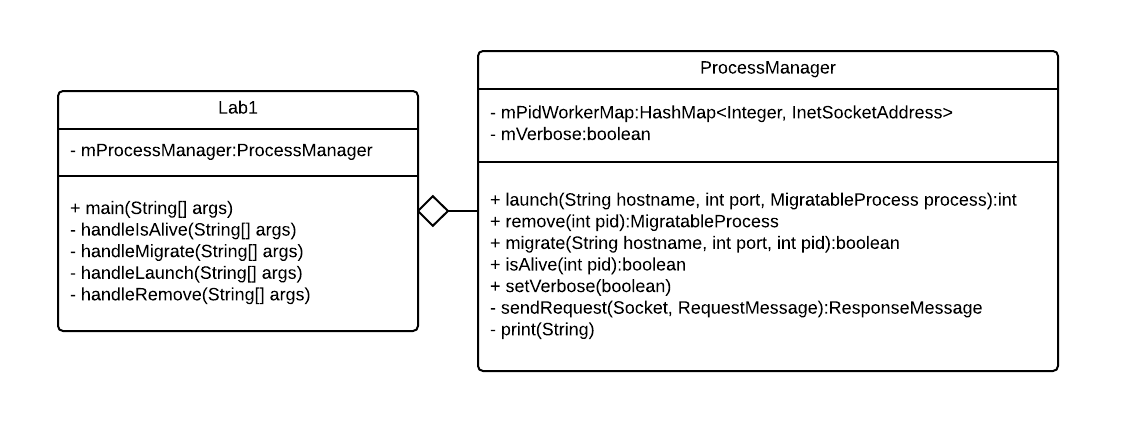
\includegraphics[scale=.4]{processManager.png}

\subsection{Worker}

The Worker class controls threads that execute given processes. Workers listen on a port given at initialization for requests from the ProcessManager. When a request comes in the Worker performs the action and sends a response.

Supported requests include
\begin{enumerate}
\item \textbf{Launch} Start the given process and respond with the process id
\item \textbf{Remove} Remove the requested process and response with a serialized version of the process or null if completed already.
\item \textbf{IsAlive} Check if the requested process is alive and respond with a boolean indicator
\end{enumerate}

\subsubsection{Design Reasoning}
One of the key insights for Workers is that there is no migrate command. Workers can treat migration as either a remove request or a launch request meaning that no migrate request is necessary. More on this will be discussed below.

The RunnablePair object is used simply as a tuple to keep track of thread and associated thread in a map that Worker maintains. Worker uses this map to keep track of living processes and which thread they are associated with.

\subsubsection{Class Diagram of Worker}
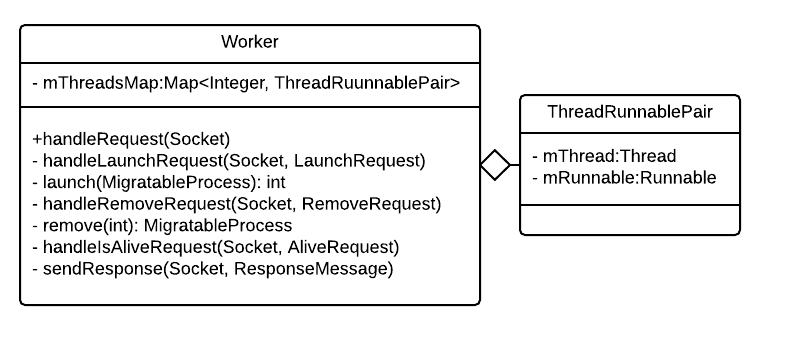
\includegraphics[scale=.4]{worker.png}

\subsection{Messages}

The ProcessManager and the Worker communicate over sockets by writing serializable objects. I created Messages as a means of setting a standard interface for the serialized objects.

Messages break down into two categories with a a number of specific message implementations in each category:
\begin{enumerate}
\item \textbf{RequestMessage} This abstract class defines messages sent from ProcessManager to Worker
	\begin{enumerate}
	\item \textbf{LaunchRequest} Contains a MigratableProcess so that it will be run by the Worker
	\item \textbf{RemoveRequest} Contains a process id to identify which process to remove
	\item \textbf{AliveRequest} Contains a process id to identify which process to poll status
	\end{enumerate}
\item \textbf{Response Message} This abstract class defines messages sent from Worker to ProcessManager
	\begin{enumerate}
	\item \textbf{LaunchResponse} Contains the process id of the started process
	\item \textbf{RemoveResponse} Contains a serialized version of the MigrateableProcess which was removed so that the process can be restarted elsewhere
	\item \textbf{AliveResponse} Contains a boolean indication of process status
	\end{enumerate}
\end{enumerate}

\subsubsection{Design Reasoning}
The message hierarchy is designed such that messages break down into logical groupings. Message, RequestMessage and ResponseMessage are all unimplementable requiring concrete request/response implementations.

When a Worker receives a request from ProcessManager it does not know the type of the request. Since there are a limited set of request types, I implemented methods for each request type that indicate the type of the request. These methods all return false in the abstract RequestMessage class so by overriding the relevant method a specific request can signal its type. For example LaunchRequest implements isLaunch() to return true.

ReponseMessage has a flag to signal success or failure. It does not however need the same type indicating methods that RequestMessage has since the ProcessManager knows what type of response to expect.

One other interesting detail is that the RemoveResponse includes a MigratableProcess. For a basic remove operation it is likely that the ProcessManager would not need the process back but this design enables the elimination of a migrate request. A migrate request is now simply a remove request followed by a launch request on the new machine. Since the remove response returns the suspended process, ProcessManager  can simply launch this process on a new machine.

\subsubsection{Class Diagram of Messages}
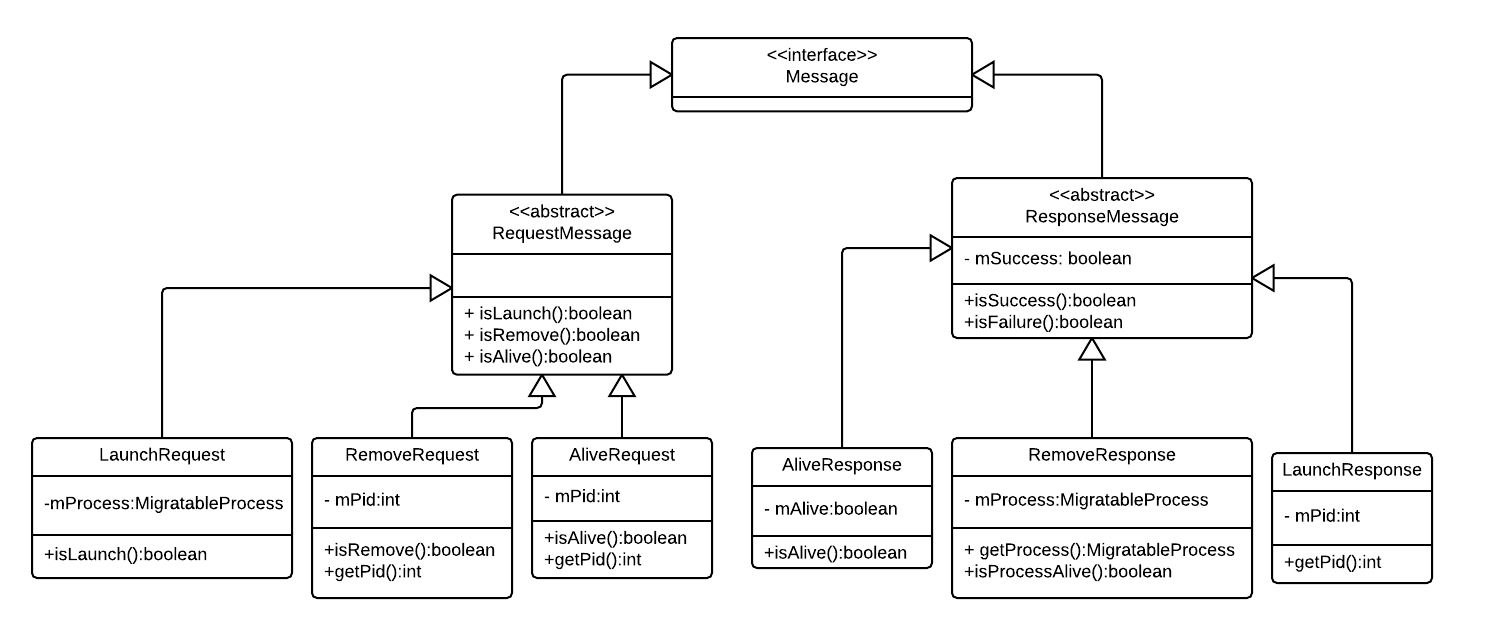
\includegraphics[scale=.3]{messages.png}

\subsection{MigratableProcess and Transactional IO}

The MigratableProcess abstract class implements process id management (getter and setter) as well as requires the creation of three methods: run, suspend and toString.

Run is used to start the given process or restart it from a suspended state. Run can contain a loop to execute code within.

Suspend places the process in a known safe state so that it can be serialized and sent over the network. Suspend works by setting a volatile flag which terminates the run loop at a safe point.

toString is used simply for debugging and print statements. toString prints the original arguments and other important details.

TransactionalFileInputStream and TransactionalFileOutputStream serve as wrappers for normal InputStream and OutputStream transactions. They open and close the stream on each transaction and keep track of file position in-between. This way once a transaction is complete the object is in a safe state and can be migrated and restarted.

\subsubsection{Design Reasoning}
A pid can only be set once. This ensures that even if restarted the process will keep the same process id.

MigratableProcess is an abstract class so as to implement the process id and its methods which are shared across all MigtratableProcess implementations.

TransactionalFileInputStream contains a readline method because I found most InputStream readers buffer their reading. Buffering causes the stream to be read into an intermediary buffer before being returned. This throws off the file position variable as the reader has read everything but the process may not have received these bytes yet. If the process then migrates this intermediary buffer is lost. Therefore I implemented my own line reader.

The suspend operation is kept the same as the example GrepProcess. I liked this implementation as it guaranteed that when a process resumed a call to run would suffice.

\subsubsection{Class Diagram of MigratableProcess and Transactional IO}
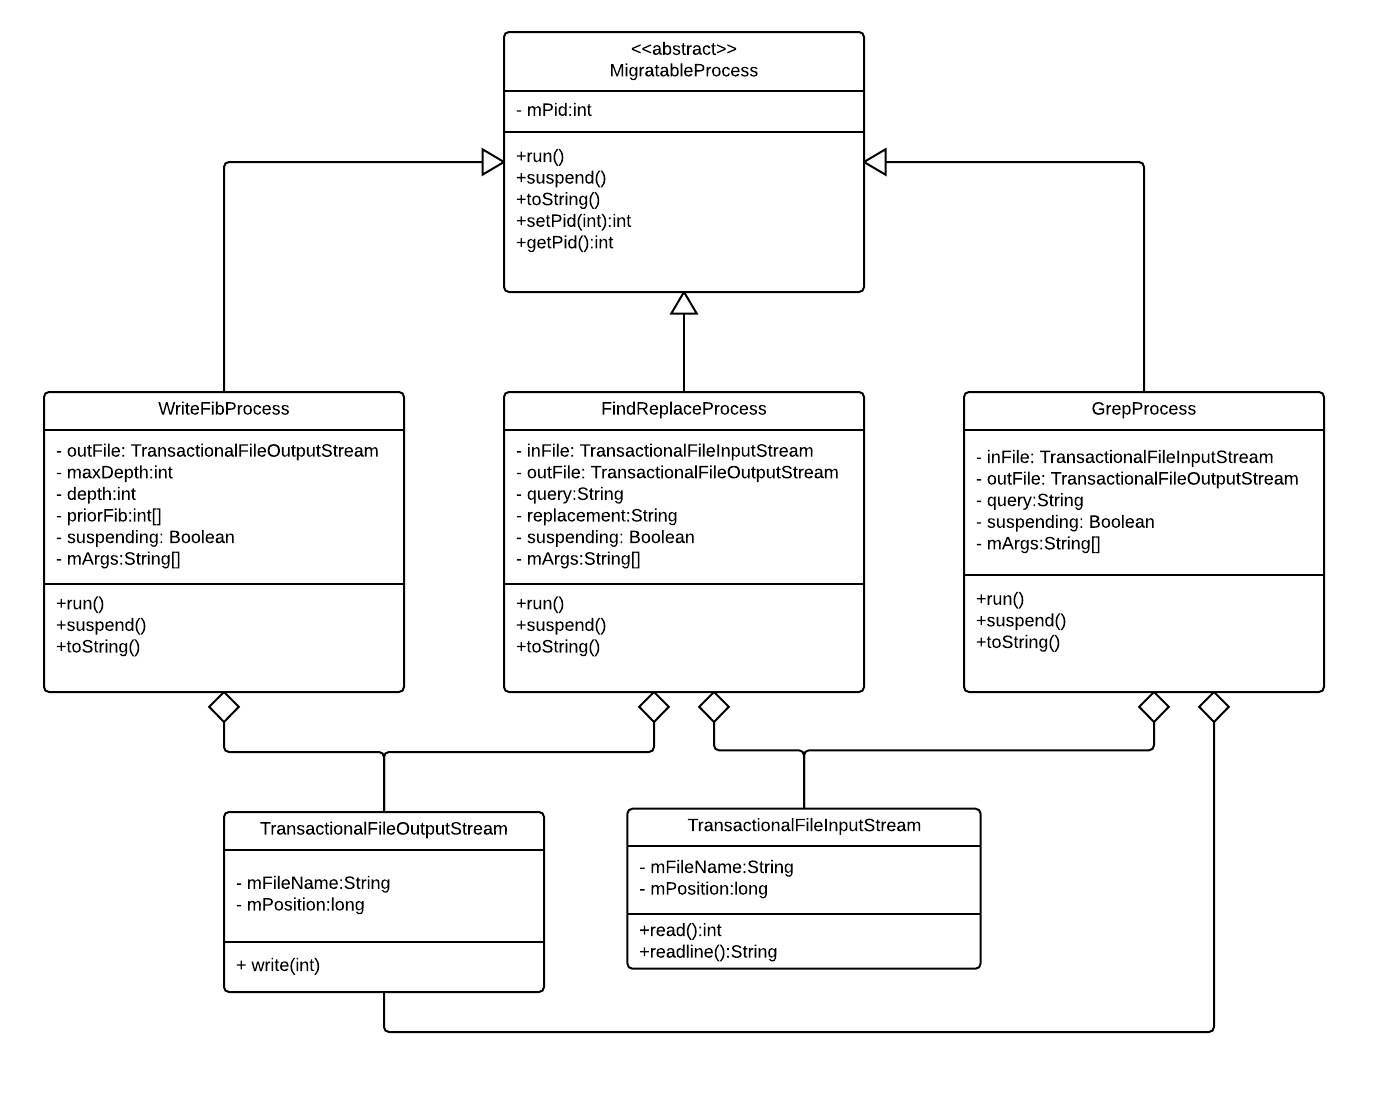
\includegraphics[scale=.3]{migratableProcess.png}

\subsection{Launch Request}

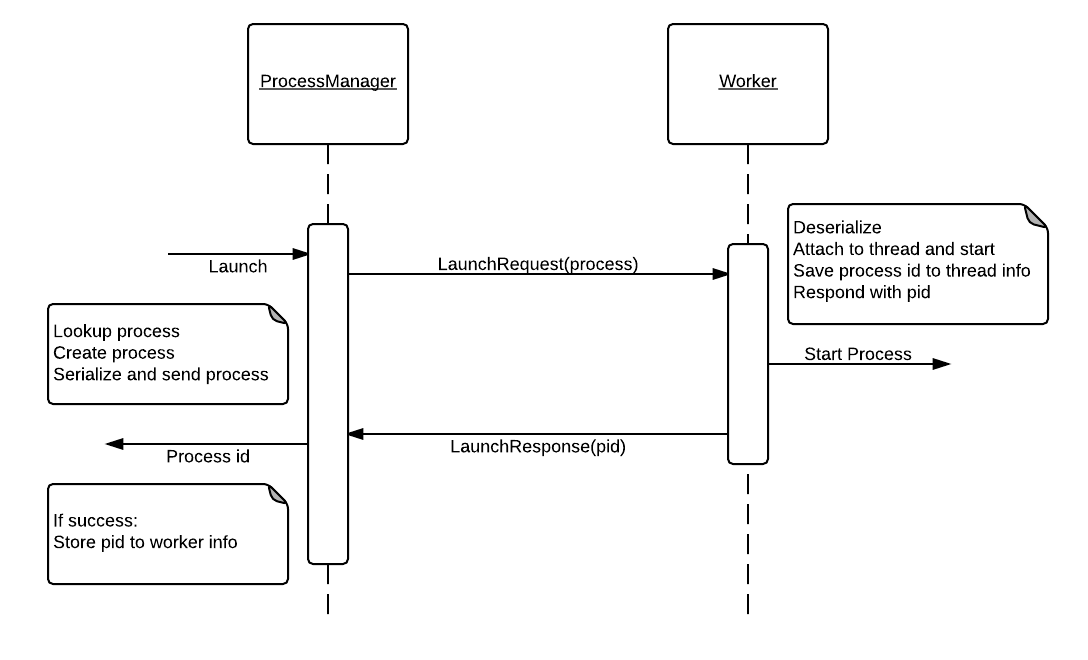
\includegraphics[scale=.4]{launch.png}

\subsection{Migrate Request}

Note that the migration can be achieved simply with a remove and a launch. This keeps the interface cleaner.

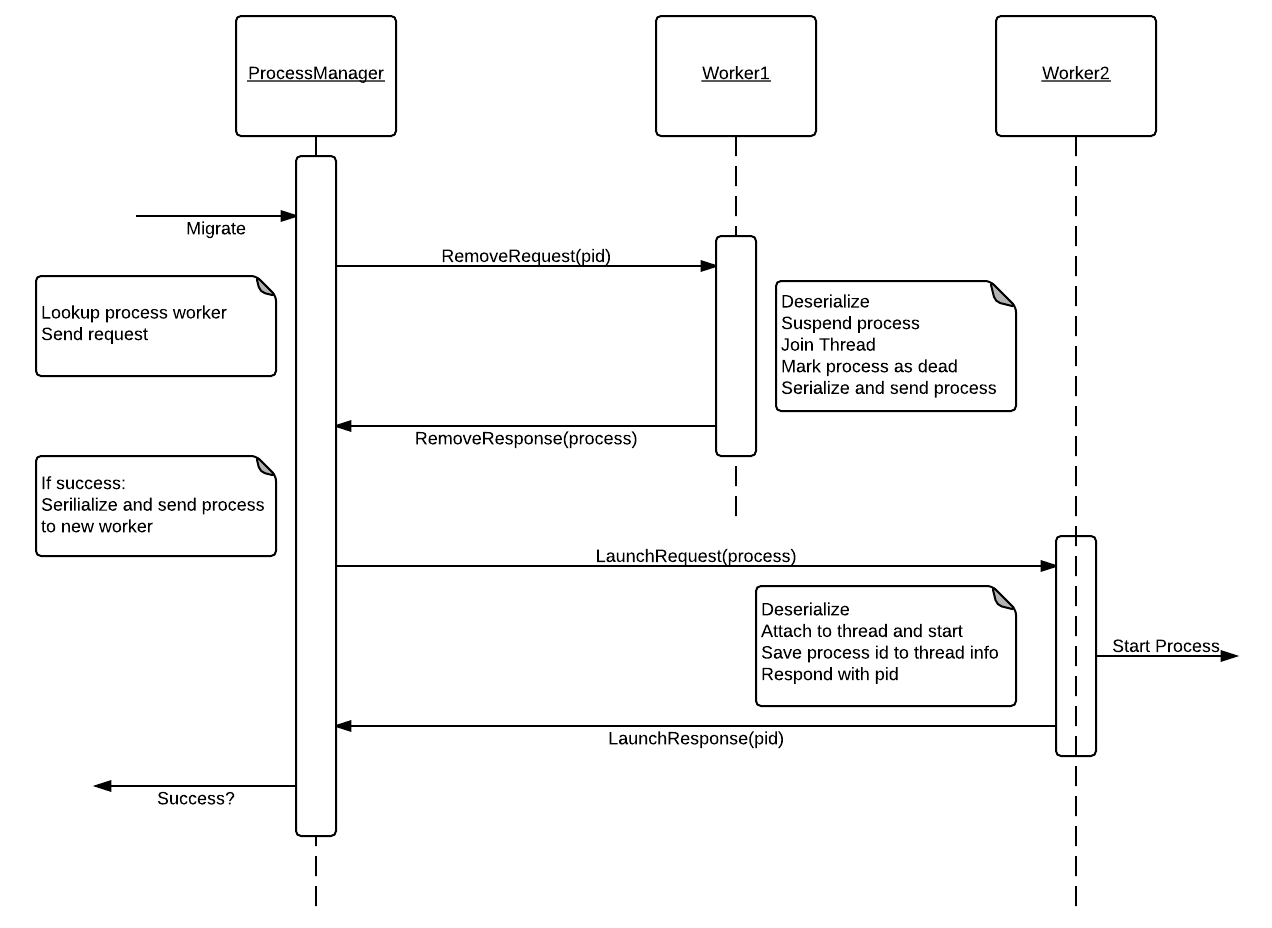
\includegraphics[scale=.3]{migrate.png}

\subsection{Remove Request}

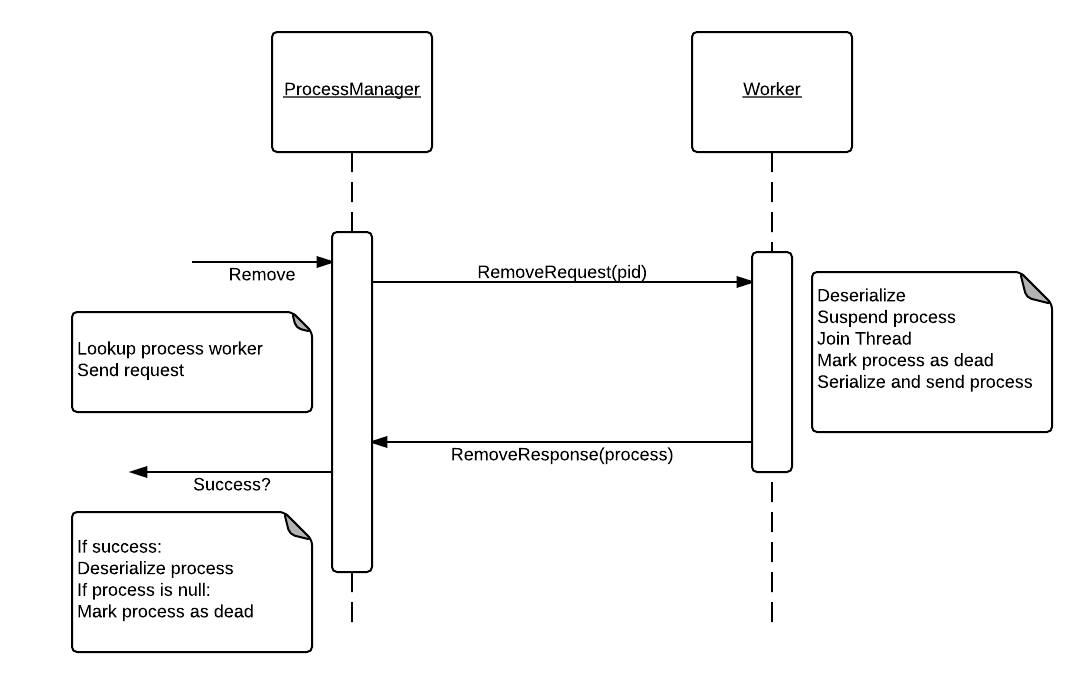
\includegraphics[scale=.4]{remove.png}

\subsection{Is Alive Request}

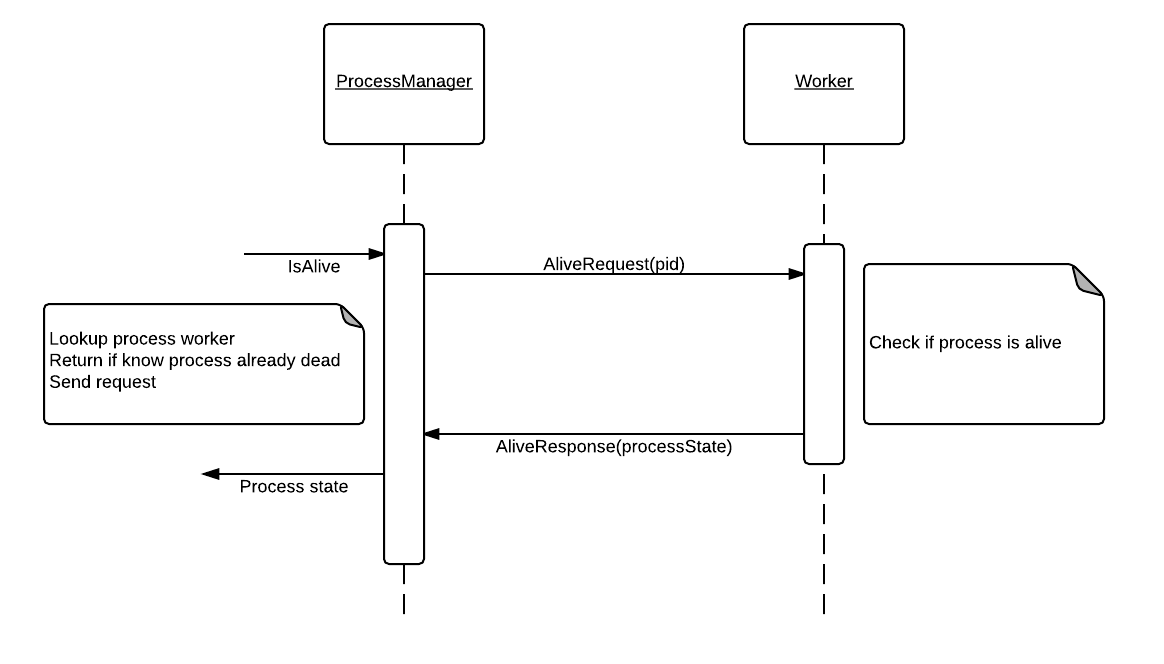
\includegraphics[scale=.4]{alive.png}


%------------------------------------------

\section{Implementation State}
The main bug that I have not determined is with the find replace process. It writes back lines with an extra newline on my computer. I believe this was an issue with the \\r character in windows but am not certain.

Other issues may arise with a very large volume of processes being run as I did not optimize for performance.

There were a few things that I would also have liked to implement:
\begin{itemize}
\item \textbf{Thread Pool} A thread pool for the Worker would be nice so that threads are not destroyed and recreated for every process.
\item \textbf{Multiple Request Handling} Currently the process manager can only handle one request at a time and blocks until a response is received. Process manager could be made multithreaded.
\item \textbf{Files stay open} Transactional i/o was implemented by closing the file after each transaction. A more efficient design would only close the file before removal.
\end{itemize}

%------------------------------------------

\section{Running the Project}

\subsection{Set-up}
\begin{enumerate}
\item Run \texttt{SETUP.py} to compile the code.
\item \texttt{cd} to \texttt{src}
\item Run \texttt{java -cp . worker/Worker <port>} with a specified port number to begin a worker. It will print its hostname which you should note for future use.
\item Run \texttt{java -cp . Lab1} to start the process manager. This will start a prompt to begin testing with.
\item In the prompt write \texttt{test} to run my tests. You will need to specify the hostname and port for two workers.
\end{enumerate}

\subsection{Example Commands}
These example commands assume that two workers have been setup on \texttt{localhost} with ports \texttt{8080} and \texttt{8081}. 

\begin{verbatim}
> launch localhost 8080 migratableprocess.GrepProcess aa grep.txt grepOut2.txt
Started process with id (1659750539)
> migrate localhost 8081 1659750539
Migrated successfully? true
> isalive 1659750539
Is process alive? true
> remove 1659750539
Remove process 1659750539
> isalive 1659750539
Is process alive? false
\end{verbatim}

%------------------------------------------

\section{Dependencies}

No dependencies beyond basic java libraries. The test cases do require that the test file be present which is how I submitted it. My tests read from \textit{test/grep.txt} for the grep process so they expect this folder and time in the path.

%------------------------------------------

\section{Testing}

You can either run my tests with the \texttt{test} command or see the earlier example on how to run processes in general. 

My processes are
\begin{itemize}
\item \texttt{migratableprocess.FindReplaceProcess} 
\item \texttt{migratableprocess.WriteFibProcess}
\end{itemize}

\end{document}
